%http://www.slideshare.net/boricles/linguistic-resources-enhanced-with-geospatial-information
In this section we present the specification of the Linked Data Life Cycle presented in \cite{Villazon_2011} as applied to linguistic resources to visualize them with geospatial information.

\subsection{Linguistics Resources}\label{sec:lr}

Our data source consists of a spreadsheet containing GPS coordinates of villages where the different Dogon languages are spoken in Mali. It also contains information about each of these languages, such as the language name, ISO 639-3 language name identifier, the language family and family code, village name, etc. and it can be easily combined via ISO 639-3 codes with dictionary data from each language. These datasets come from the Dogon Languages Project and are freely available online.\footnote{\url{http://dogonlanguages.org}} Each set of data points per village is associated with a GPS coordinate and can thus be plotted on a world map. Because the set of Dogon languages that belong to the Dogon language family have been until recently poorly documented and described, information about where these languages are spoken in relation to each other can assist linguists in identifying the genealogical relatedness of these languages. The visualization of linguistic information on maps has been a successful method for generating and testing hypotheses (cf.\ \cite{Haspelmath_etal2008}).

%Steve going to need your help here. 

\subsection{Specification}
The process of publishing Linked Data has an iterative incremental life cycle model. Data sources must be identified and analyzed and entities in the data must be assigned a URI. A key element of Linked Data is also the ability to reuse and leverage data that has already been published as Linked Data. By identifying the schema of resources that are to be transformed into Linked Data, conceptual components and their relationships can be properly modeled into the RDF triple format. In the Dogon GPS spreadsheet, we were able to identify fields such as language name, ISO 639-3 code, language family and subfamily, alternative languages spoken in each village, village names, municipality, notes about the speaker's society, and geospatial information and assign them a URI. See Fig.\ \ref{spreadsheet}.

\begin{figure*}[b!hpt]
\caption{Data that contains villages in Mali with language information}\label{spreadsheet}
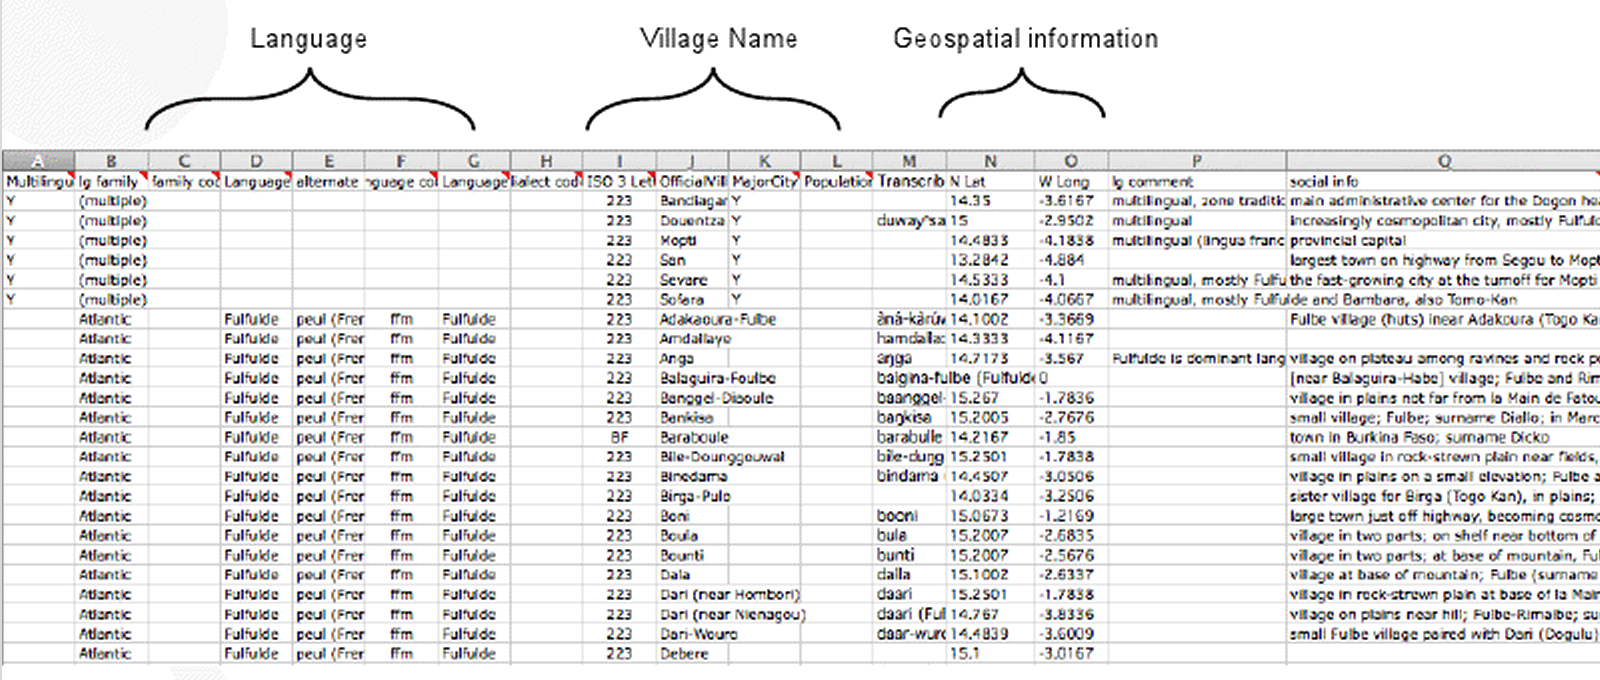
\includegraphics[width=15cm]{img/spreadsheet.png}
\end{figure*}

All resources in the dataset are given dereferenceable URIs and we've attempted to use meaningful names instead of opaque ones. We also reuse URIs where we can, including using the General Ontology of Linguistic Description (GOLD) for morphosyntactic data descriptions \cite{farrar2003linguistic}.\footnote{ \url{http://linguistics-ontology.org/}.} The base URI structure uses the \surl{http://linguistic.linkeddata.es/} namespace. Vocabulary elements are appended with \surl{/ontology/{property|class}} and instances with \surl{/dataset/resource/{r. type|r. name}}. We also reused URIs from the WGS84 Geo Basic Vocabulary for the representation of geospatial data.\footnote{\url{http://www.w3.org/2003/01/geo/}} 

\subsection{RDF Generation}
Next, the spreadsheet data was transformed into RDF. First we imported the spreadsheet into MySQL. Then we defined a set of R2RML mappings. R2RML is a RDF-to-RDF mapping language and we used it to creat mappings between elements in the MySQL database table from the spreadsheet and the RDF vocabulary that we defined.\footnote{\url{http://www.w3.org/TR/r2rml/}} Lastly, using the R2RML engine and morph,\footnote{\url{https://github.com/boricles/morph}} we generated the RDF instances using the R2RML defined mappings.

\subsection{Publication}\label{sec:pub}
The RDF data that we generated is stored in a triple store with the Virtuoso software, which we use to publish the data online.\footnote{\url{http://virtuoso.openlinksw.com/}} Integrated with Pubby,\footnote{\url{http://www4.wiwiss.fu-berlin.de/pubby/}} Virtuoso allows us to leverage content management to serve up machine-readable and human consumable webpages that contain information about each village, such as which languages are spoken there, where the village is located, additional information about the society, etc.\footnote{See for example the page on the village Boni: \url{http://linguistic.linkeddata.es/page/mlode/resource/Village/Boni}.} Virtuoso also provides a SPARQL endpoint with which we can query and share the data.

% Virtuoso integrates with Pubby\footnote{\url{http://www4.wiwiss.fu-berlin.de/pubby/}} to publish the results - Pubby is a fronted for endpoints, allowing users to query the data in the Virtuoso server using the SPARQL query language. Once Virtuoso and Pubby are running on data that has been loaded in using the R2RML engine, all of the data is essentially available for humans and computers to read. At this point the data, if it has been specified correctly, if the URIs are HTTP resolvable and if the vocabulary followed set standards, the process of lifting data into the Semantic Web is practically done.  What's left is actually exploiting this data. 

% The generated RDF was then stored in Virtuoso\footnote{\url{http://virtuoso.openlinksw.com/}} open source version. Virtuoso is essentially the server, allowing the RDF data loaded in the Generation step above to be queried using an endpoint. Virtuoso integrates with Pubby\footnote{\url{http://www4.wiwiss.fu-berlin.de/pubby/}} to publish the results - Pubby is a fronted for endpoints, allowing users to query the data in the Virtuoso server using the SPARQL query language. Once Virtuoso and  Pubby are running on data that has been loaded in using the R2RML engine, all of the data is essentially available for humans and computers to read. At this point the data, if it has been specified correctly, if the URIs are HTTP resolvable and if the vocabulary followed set standards, the process of lifting data into the Semantic Web is practically done.  What's left is actually exploiting this data. 

\subsection{Exploitation}
Following the previous steps of specification, RDF generation and publication, we expose the RDF data, enhanced with GPS coordinates, using map4rdf.\footnote{\url{https://github.com/boricles/linked-data-visualization-tools}} map4rdf is a maps viewer of RDF resources with geometrical information built on OpenStreetMap\footnote{\url{http://www.openstreetmap.org/}} and it can be used to visualize information in RDF datasets. Additionally, it is extensible with Google app plugins. The parameters of map4rdf must be set so that the application knows where to locate the endpoint of Dogon data in RDF (that we set up with Virutoso) and which geometry model that we are using (since there different standards for geo-mapping). With the parameters set, a user can open the map4rdf application in his or her web browser and explore the location of villages where Dogon are spoken.\footnote{The map4rdf instantiation for the Dogon villages resides at: \url{http://geo.linkeddata.es/map4rdf-dogon/}.} Fig.\ \ref{fig:map4rdf} provides an illustration.

\begin{figure*}[htb!p]
\centering
%\includegraphics[scale=0.45]{IMGS/detalle_bn.png}
%\includegraphics[width=0.70\textwidth]{IMGS/detalle.pdf}
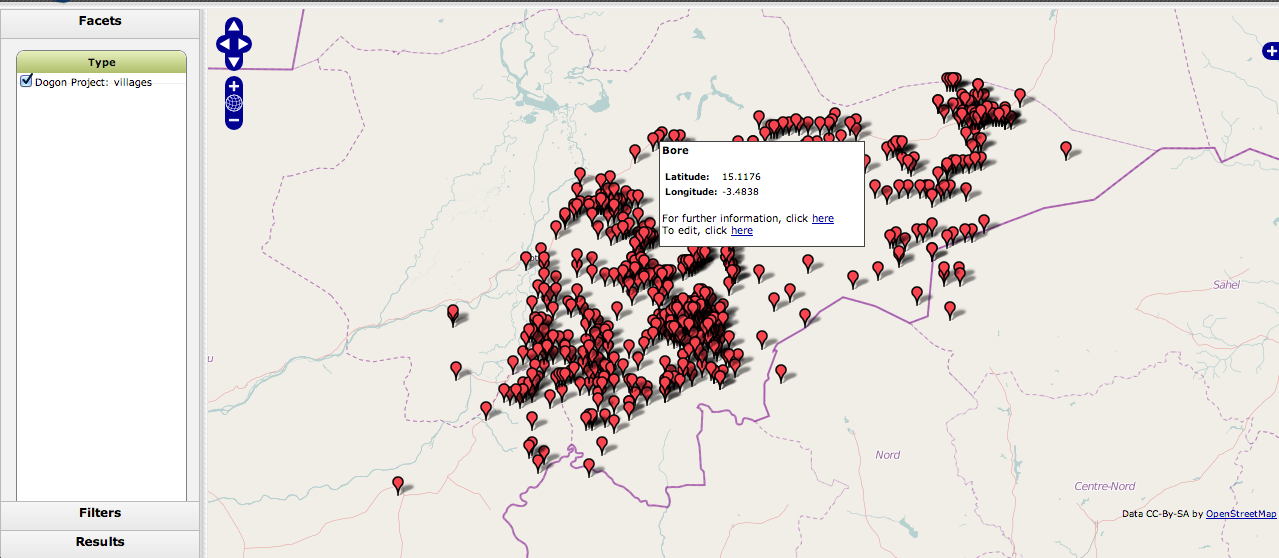
\includegraphics[width=0.99\textwidth]{img/map4rdf.png}
\caption{Visualization of the Dogon villages}
\label{fig:map4rdf}
\end{figure*}

Each point on the map comes from GPS coordinates in the original spreadsheet, which have been transformed into RDF triples and stored in a triple store with Virtuoso. This triple store can be queried with SPARQL or its endpoint can be given as an endpoint for programs like map4rdf to access its data contents.  Each pin in Fig.\ \ref{fig:map4rdf} can be clicked on, showing the village name, its latitude and longitude, and a link for more information about the language. This is shown in Fig.\ \ref{pin.png}.

\begin{figure*}[htb!p]
\centering
%\includegraphics[scale=0.45]{IMGS/detalle_bn.png}
%\includegraphics[width=0.70\textwidth]{IMGS/detalle.pdf}
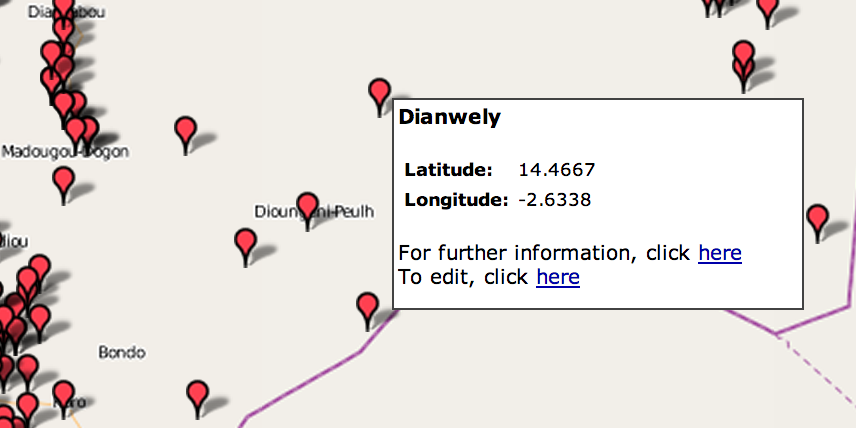
\includegraphics[width=0.99\textwidth]{img/pin.png}
\caption{Clicking on a pin}
\label{pin.png}
\end{figure*}

When clicking on the link for more information, a request is sent to the SPARQL endpoint for all information in the RDF triple store about that particular village. When accessing the data through map4rdf, the endpoint knows through content management to return an HTML page that displays the query results, as shown in Fig.\ \ref{more_information.png}.

\begin{figure*}[htb!p]
\centering
%\includegraphics[scale=0.45]{IMGS/detalle_bn.png}
%\includegraphics[width=0.70\textwidth]{IMGS/detalle.pdf}
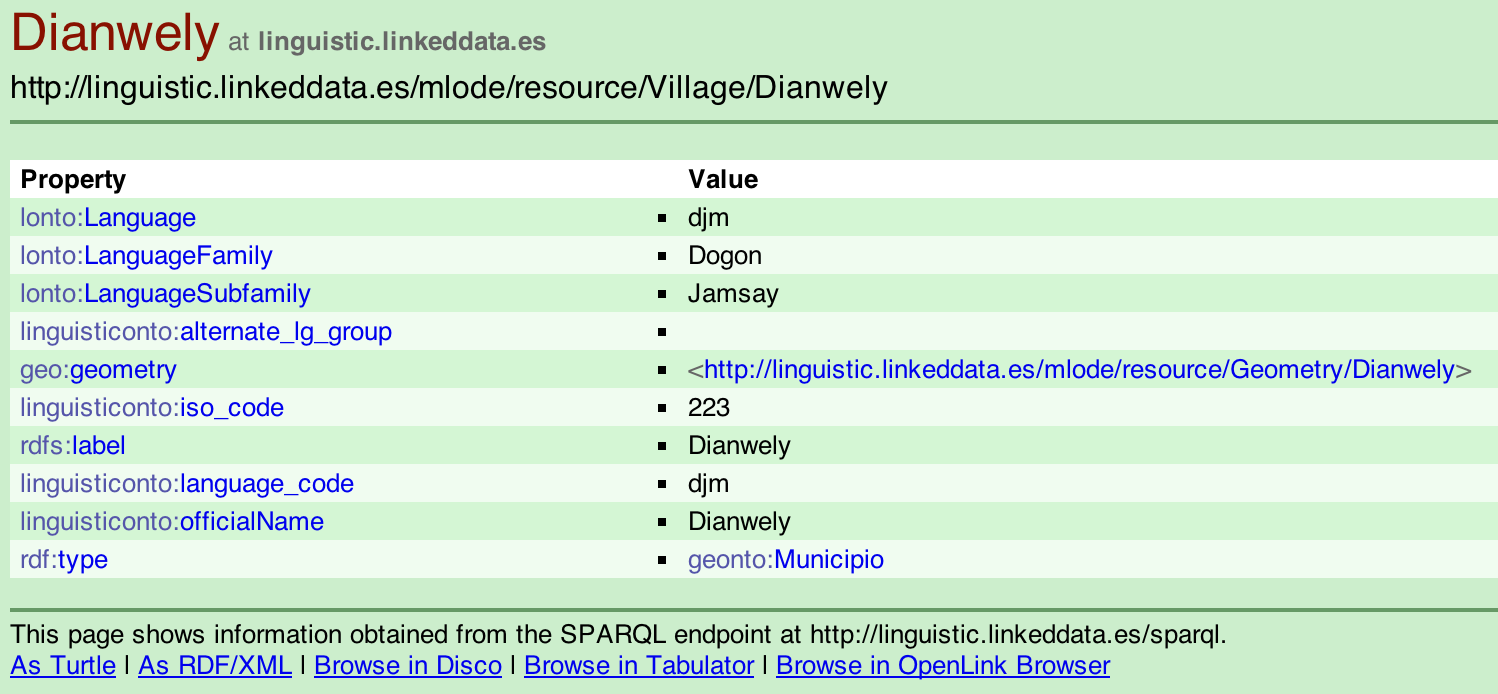
\includegraphics[width=0.99\textwidth]{img/more_information.png}
\caption{More information about a village}
\label{more_information.png}
\end{figure*}

